\documentclass[10pt,a4paper]{article}
\usepackage[utf8]{inputenc}
\usepackage{polski}
\usepackage{amsmath}
\usepackage{amsfonts}
\usepackage{amssymb}
\usepackage{graphicx}
\usepackage{verbatim}
\author{Korzeniowski Wojciech, Gadawski Łukasz}
\title{Wyznaczenie sumarycznie najkrótszych ścieżek rozłącznych krawędziowo \\
	Sprawozdanie 3}
\begin{document}
\maketitle

\section{Cel projektu}
Realizacja projektu polegała na zaimplementowaniu zmodyfikowanej wersji algorytmu Dijkstry, która umożliwia znalezienie dwóch rozłącznych krawędziowo ścieżek w skierowanym grafie dla dowolnej pary wierzchołków.

Jednym z praktycznych zastosowań wyznaczanie najkrótszych rozłącznych krawędziowo ścieżek w grafie może być chęć poprawy niezawodności sieci przesyłowych poprzez wykorzystanie najbardziej optymalnych ścieżek jako zapasowyh ścieżek. Innym z zastosowaniem może być podział transmisji danych pomiędzy dwie ścieżki dzięki podczas wystąpienia awari możliwa jest częściowa transmisja danych.

\section{Struktury danych}
W programie wykorzystane są następujące struktury:
\begin{itemize}
	\item Vertex - reprezentuje wierzchołek, zawiera nazwę.
	\item Edge - reprezentuje krawędź skierowaną, zawiera wierzchołek początkowy, wierzchołek końcowy, wagę krawędzi.
	\item Graph - reprezentuje graf, zawiera zbiór krawędzi oraz zbiór wierzchołków	należących do grafu.
	\item GraphPath - reprezentuje ścieżkę w grafie, zawiera listę krawędzi.
\end{itemize}

\section{Opis algorytmu}
Poniżej przedstawiony został przebieg wykonania algorytmu w celu znalezienie dwóch rozłącznych krawędziowo ścieżek.

\begin{enumerate}
\item Znajdź najkrótszą ścieżkę przy pomocy standardowego algorytmu Dijkstry.
\item Dla każdej krawędzi znalezionej ścieżki odwróć jej zwrot oraz zmień wagę na ujemną.
\item Ponownie znajdź najkrótszą ścieżkę w tak otrzymanym grafie, tym razem korzystając ze zmodyfikowanej wersji algorytmu Dijkstry. (opis \ref{modif})
\item Ze zbioru reprezentującego sumę zbiorów krawędzi znalezionej ścieżki usuń część wspólną.
\item Z pozostałego zbioru krawędzi znajdź iteracyjnie ścieżki idąc od wierzchołka końcowego ku początkowemu usuwając przy tym krawędzie zużyte z wynikowego zbioru.
\item Zwróc uzyskane ścieżki.
\end{enumerate}
\subsection{Zmodyfikowany algorytm Dijkstry}
\label{modif}
Oznaczenia: \\ \\
$S$ - wierzchołek startowy \\
$D$ - wierzchołek docelowy \\ 
$neighbour(S)$ - zbiór wierzchołków sąsiadujących z $S$ \\
$distance(A)$ - odległość od wierzchołka startowego $S$ do wierzchołka $A$ \\
$predecessor(A)$ - tablica zawierająca poprzednik wierzchołka $A$ dla znalezionej ścieżki \\
$cisited$ - zbiór wierzchołków odwiedzonych przez algorytm \\
$searchNodes$ - zbiór wierzchołków do wyszukania najkrótszej ścieżki \\ \\

Kroki algorytm: 
\begin{enumerate}
\item Dla każdego wierzchołka $V \in v $ przypisz $distance(V)=+\inf$.
\item Dla wierzchołka startowego przypisz $distance(S)=0$.
\item Dla każdego $NS \in neighbours(S)$ przypisz $distance(NS)=weight(S,NS)$ oraz $predecessor(NS)=S$.
\item Dodaj sąsiadów wierzchołka $S$ do zbioru wierzchołków do przeszukania $searchNodes.add(neighbour(S))$.
\item Znajdź $F \in searchNodess$ dla którego wartość $distance(F)$ jest najminejsza.
\item Usuń wierzchołek $F$ ze zbioru wierzchołków do przeszukania $searchNodes.remove(F)$.
\item Jeżeli $F=D$ to ZAKOŃCZ
\item Dla każdego wierzchołka $NF \in neighbour(F)$ jeżeli $distance(F) + weight(F,NF)<distance(NF)$ przypisz nową, krótszą odległość $distance(ND)=distance(F)+weight(F, NF)$ oraz nowego poprzednika $predecessor(NF)=F$ oraz dodaj wierzchołek do zbioru przeszukania $searchNodes.add(NF)$.
\end{enumerate}


\section{Przebieg działania aplikacji}
W ramach projektu została stworzona aplikacja udostępniające następujące funkcjonalności.
\subsection{Wykonanie na podstawie danych z pliku tekstowego}
Umożliwia wyznaczenie dwóch rozłącznych krawędziowo ścieżek na podstawie własnego, zdefiniowanego grafu w pliku tekstowym o następującej strukturze:
\verbatiminput{simpleGraph.txt}

gdzie komentarz rozpoczyna się od znaku \#, każda linia reprezentuję pojedynczą krawędź rozpatrywanego grafu przy czym pierwsza kolumna opisuję etykietę wierzchołka początkowego danej krawędzi, kolumna druga definiuje etykietę wierzchołka końcowego, a w ostatniej kolumnie znajduje się waga konkretnej krawędzi. Wynik działania algorytmu będą reprezentowały listy etykiet wierzchołków najkrótszych ścieżek jeśli takie będą istniały oraz wagi konkretnych ścieżek.

\subsection{Generowanie grafu}
Funkcjonalność umożliwiająca podanie liczby wierzchołków oraz krawędzi oraz na tej podstawie wygenerowaniu przykładowego grafu. Następnie dla tak uzyskanego grafu następuje wyznaczenie dwóch najkrótszych ścieżek rozłącznych krawędziowo, wypisanie tych ścieżek na konsoli oraz wizualizacja graficzna takiego grafu.
\subsection{Uruchomienie benchmarku}
Ponadto aplikacja umożliwia dla wygenerowanego grafu na podstawie liczby wierzchołków oraz krawędzi wyznacznie ilości iteracji algorytmu potrzebnych do wyznaczenia rozłącznych ścieżek dla takiego przykładowo wygenerowanego grafu.

\section{Kryteria stopu}
Kryteriami stopu w rozpatrywanym algorytmie są osiągnięcie wierzchołka końcowego podanego na wejściu programu lub przejrzenie całej listy wierzchołków 'nieprzejrzanych' w kontekście wykonywanego zmodyfikowanego algorytmu Dijkstry.

\section{Testy poprawności działania algorytmu}
Poniżej zostały zamieszczone przykładowe wyniki wywołania programu dla zadanych wierzchołków w celu zbadania poprawności działania algorytmu.
\subsection{Wejście programu}
\verbatiminput{test1.txt}

\subsection{Wyjście pgoramu}
Program przedstawia dwie ścieżki sumarycznie najkrótsze i rozłączne krawę-
dziowo oraz sumaryczną wagą ścieżki. Wyjściem programu dla przedstawionego wyżej wejścia jest: \\
\subsection{Przypadek testowy 1}
$A \quad-> B\quad (5)$ \\
$A \quad-> C \quad(10)$ \\
$A \quad-> D\quad (20)$ \\
$B \quad-> D \quad(18)$\\
$C \quad-> E\quad (5)$\\
$C \quad-> I\quad (100)$\\
$D \quad-> E\quad (10)$\\
$D \quad-> F \quad(50)$\\
$D\quad -> H \quad(70)$\\
$E \quad-> F \quad(3)$\\
$E \quad-> G \quad(30)$\\
$E \quad-> H\quad (10)$\\
$F\quad -> G\quad (25)$\\
$F\quad -> H \quad(10)$\\
$G\quad -> I\quad (10)$\\
$H \quad-> I\quad (3)$\\

Oczekiwany wynik dla $ A\quad -> I:$
\begin{itemize}
	\item $A \quad-> C \quad-> E \quad-> H \quad-> I \quad(28)$
	\item  $A \quad-> D \quad-> E\quad -> F \quad-> G \quad-> I \quad(68)$
\end{itemize}

\subsection{Przypadek testowy 2}
$A\quad -> B (1)$\\
$A \quad-> E (5)$\\
$A \quad-> F (2)$\\
$B \quad-> C (1)$\\
$B\quad -> E (2)$\\
$C \quad-> D (3)$\\
$E \quad-> D (3)$\\
$F \quad-> C (1)$\\
$F\quad -> D (6)$\\

Oczekiwany wynik:\\
\begin{itemize}
	\item $ A \quad -> \quad B -> E\quad -> D (6)$
	\item $ A \quad-> F\quad -> C\quad -> D (6)$\\
\end{itemize}

\subsection{Przypadek testowy 3}
$A\quad -> B \quad(2)$\\
$A\quad -> C\quad (1)$\\
$A \quad-> I\quad (5)$\\
$B\quad -> C\quad (6)$\\
$C \quad-> D\quad (1)$\\
$C\quad -> E\quad (1)$\\
$D \quad-> E\quad (2)$\\
$D\quad -> F \quad(2)$\\
$E \quad-> F \quad(1)$\\
$E \quad-> K \quad(3)$\\
$F\quad -> G\quad (1)$\\
$F \quad-> I\quad (1)$\\
$F\quad -> J \quad(1)$\\
$F\quad -> K \quad(1)$\\
$G\quad -> H \quad(1)$\\
$I\quad -> E \quad(1)$\\
$I \quad-> J \quad(5)$\\
$J \quad-> H \quad(1)$\\
$K\quad -> H\quad (5)$\\

Oczekiwany wynik dla $A \quad -> H:$\\
\begin{itemize}
	\item $ A\quad -> C\quad -> D\quad -> F \quad-> G\quad -> H\quad (6)$
	\item $ A \quad-> I\quad -> E \quad-> F \quad-> J\quad -> H \quad(9)$
\end{itemize}


\section{Sytuacje awaryjne}
W przypadku gdy nie istnieją dwie, rozłączne krawędziowo ścieżki pomiędzy wybranymi wierzchołkami, program zwróci odpowiedni komunikat informujący o tym użytkownika.


\section{Testy wydajnościowe}
Tabela \ref{fig:time-cons} przedstawia czas wykonania zaimplementowanego algorytmu w zależności od wielkości grafu. Wiersze reprezentują ilość wierzchołków ze skokiem $V_{i} = V_{i-1}^{1.05}$ oraz liczba krawędzi z mnożnikiem $E_{i} = 1.3 * E_{i-1}$. Wartości zostały dobrane arbitralnie na potrzeby uzyskania reprezentatwnych wyników. Na rysunku w każdej komórce występuje wartość mediany 10 wykonań algorytmu. Mediana pozwala na uzyskanie bardziej realnych wyników w porównaniu ze średnią z uwagi na mniejszą wrażliwość na odchylenia występujące w próbach.

\begin{figure}[H]
	\centering
	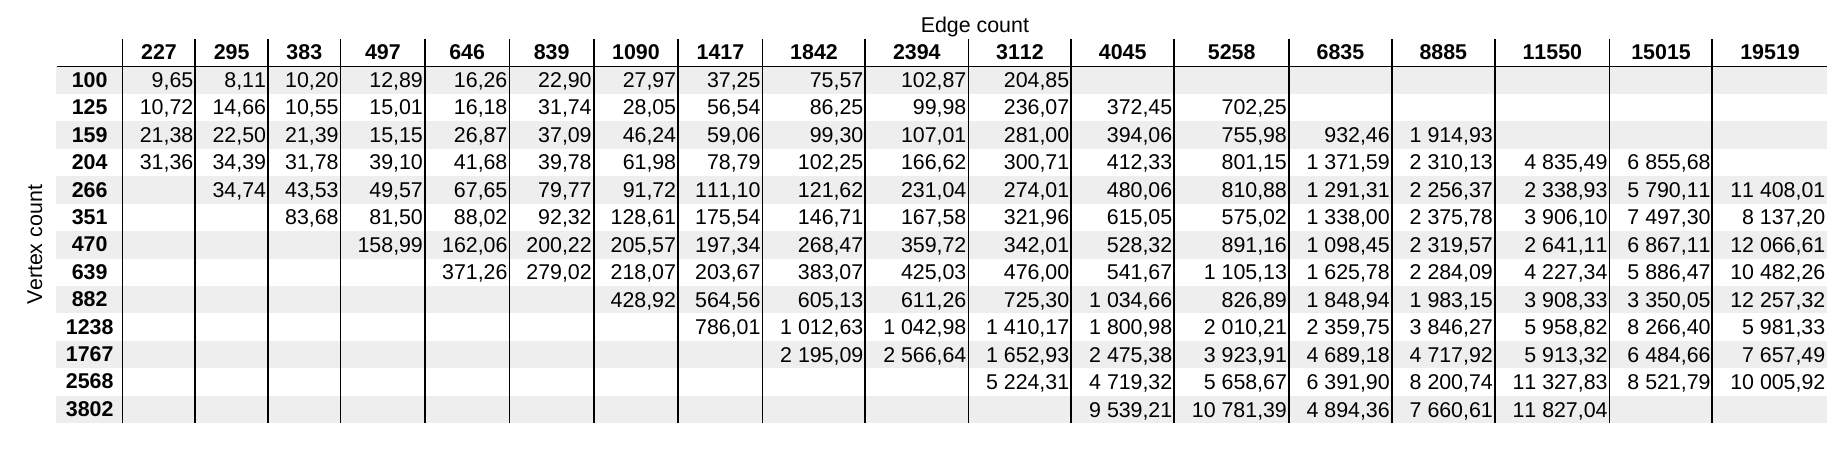
\includegraphics[scale=0.3]{time-cons}
	\caption{Czas wykonania.\label{fig:time-cons}}
\end{figure}

\section{Analiza złożoności obliczeniowej}
Złożoność obliczeniowa algorytmu Dijkstry wynosi $O(E * \ln V)$, w naszym przypadku założylismy, że jego zmodyfikowana wersja będzie miała podobną złożoność. W obu poniższych tabelach główne wartości reprezentuje wartość mediany.

Rysunek \ref{fig:edge-element} przedstawia analizę czasu wykonania algorytmu pod względem ilości krawędzi w grafie. W celu zbadania poprawności tej analizy potrzeba sprawdzić zgodność podanej proporcji pomiędzy wykonaniami dla kolejnych ilości krawędzie, a wartością oczekiwaną równą 1.3, która reprezentuje oczekiwany przelicznik złożoności w miarę proporcjonalnego zwiększania ilości krawędzi. Jak widac mediana tego przelicznika wynosi wartość 1.283 co jest bardzo zbliżoną wartością do wartości oczekiwanej.

\begin{figure}[H]
	\centering
	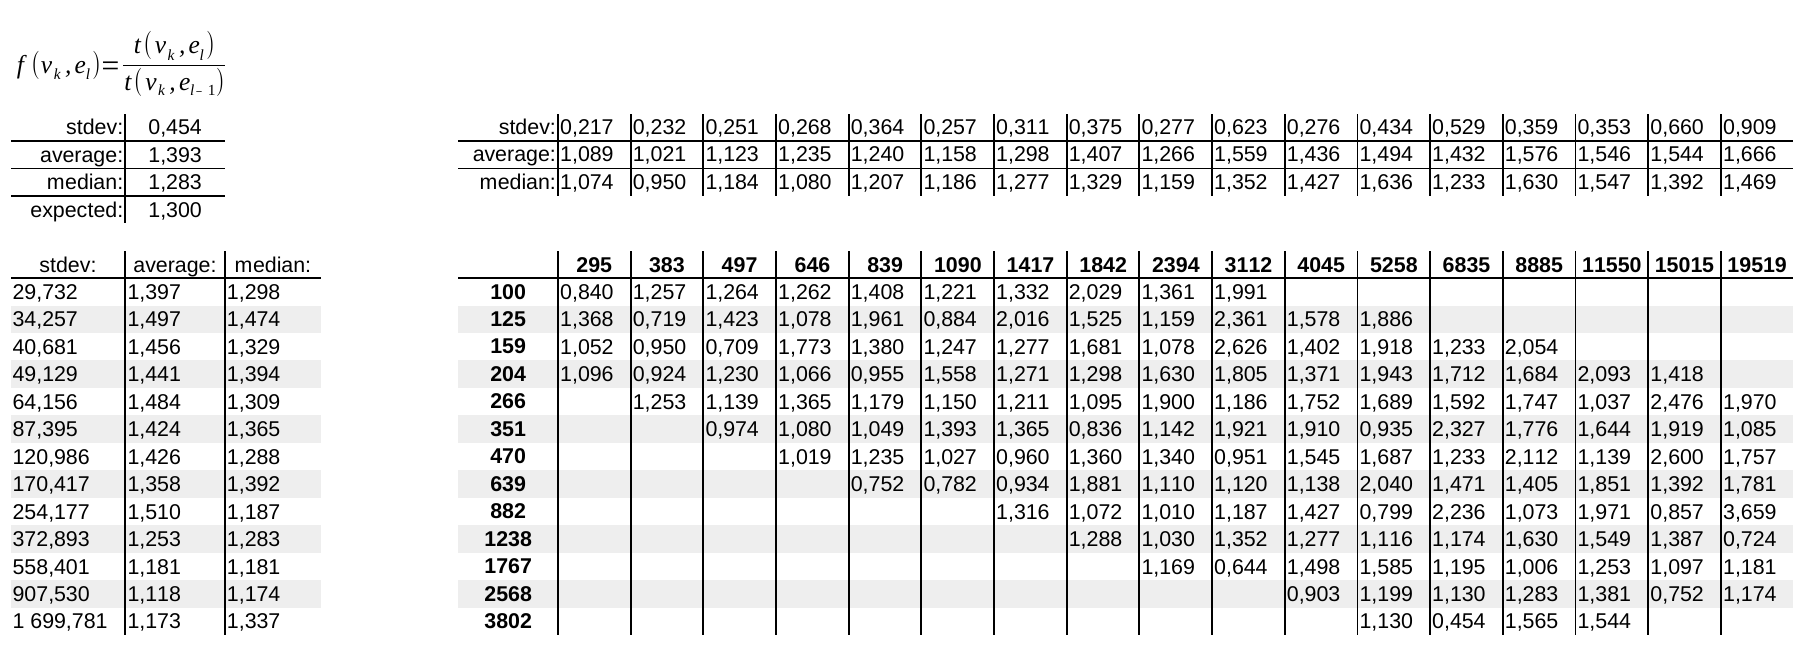
\includegraphics[scale=0.3]{edge-element}
	\caption{Analiza ze względu na ilość krawędzi.
			\label{fig:edge-element}}
\end{figure}


Rysunek \ref{fig:vertex-element} przedstawia analizę czasu wykonania algorytmu pod względem ilości wierzchołków w grafie. W tym przypadku badane są proporcje odpowiednich logarytmów naturalnych. Wartością oczekiwaną w tym przypadku jest 1.05, natomiast wartością mediany uzyskaną na podstawie próbek jest 0.959, co jest wartością lekko rozbieżną. Jednakże, po analizie wartości mediany widać, że jej wartość wzrasta wraz z ilością wierzchołków i taka rozbieżność może wynikać ze zbyt małych prób wykorzystanych w tej analizie.

\begin{figure}[H]
	\centering
	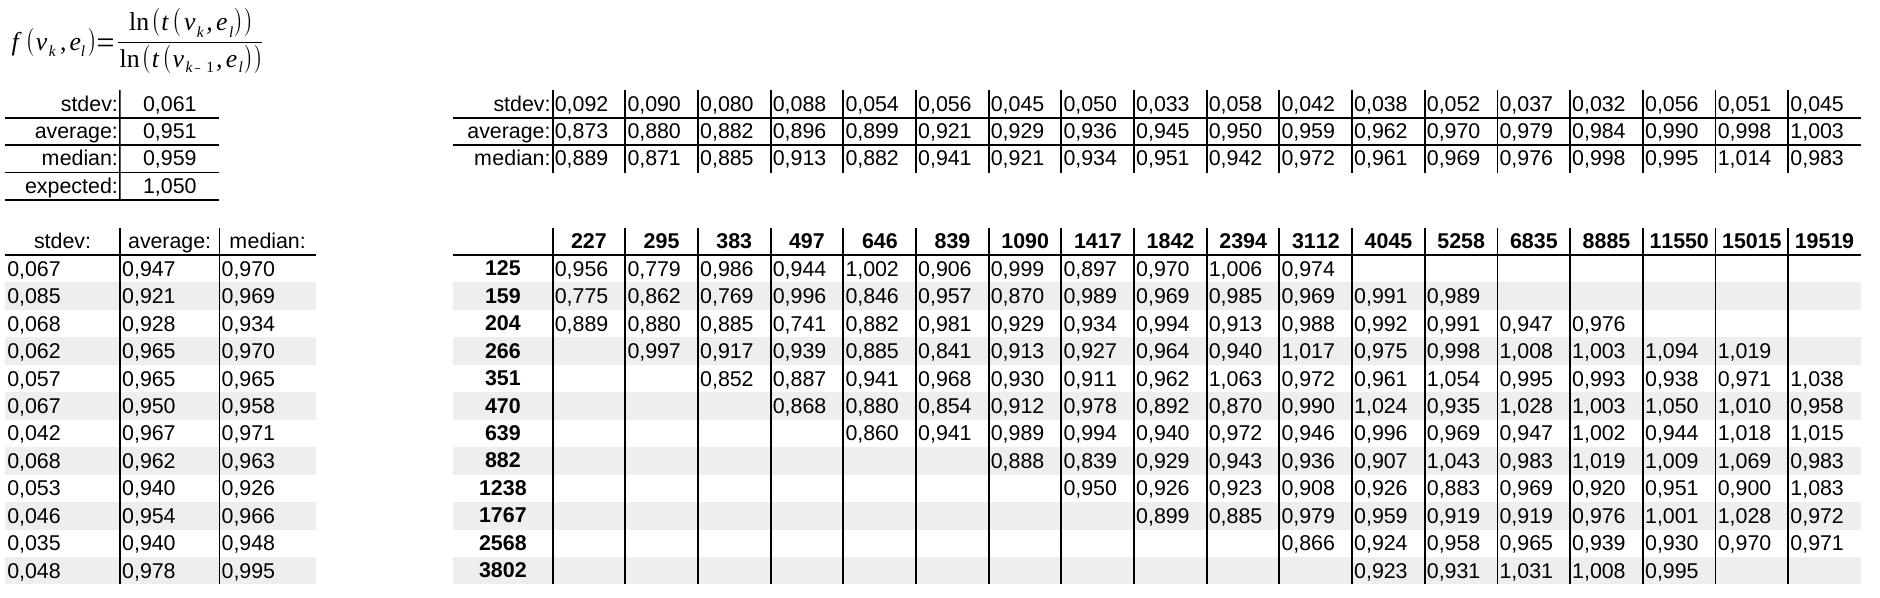
\includegraphics[scale=0.3]{vertex-element}
	\caption{Analiza ze względu na ilość wierzchołków.	\label{fig:vertex-element}}
\end{figure}


\end{document}